\begin{figure}[H]
\centering
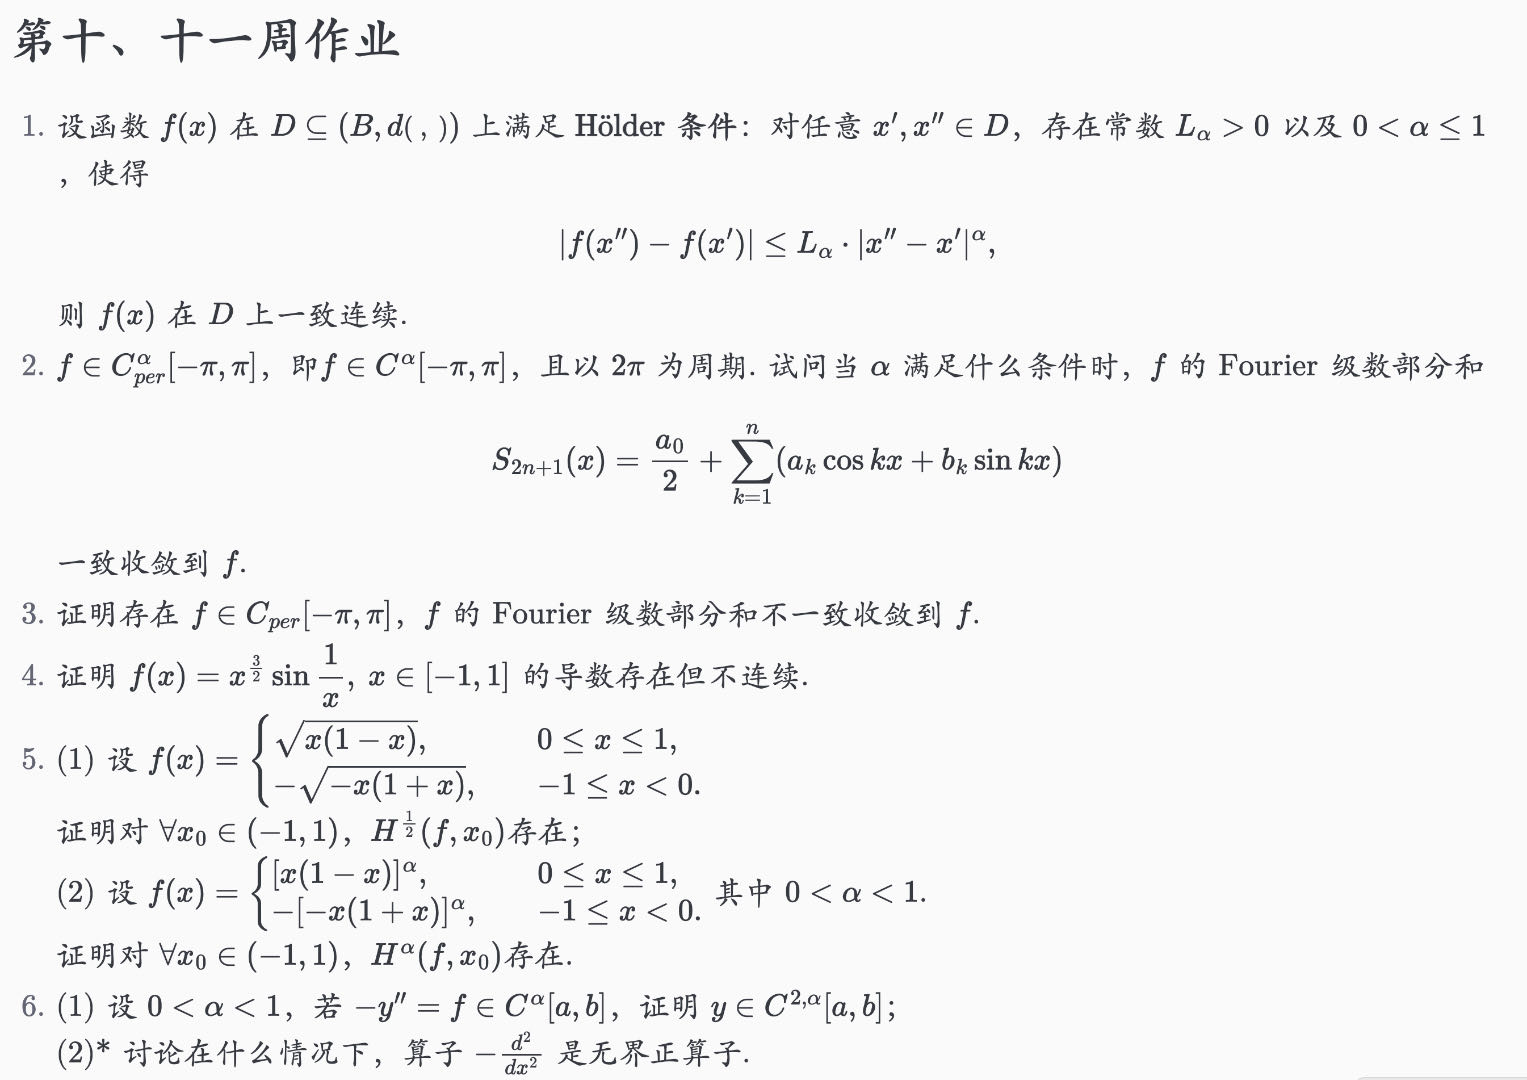
\includegraphics[width=\textwidth]{6498218cd114e8c64311afd79fffef67.jpg}
% \caption{}
\label{}
\end{figure}

\begin{exercise}
\begin{figure}[H]
\centering
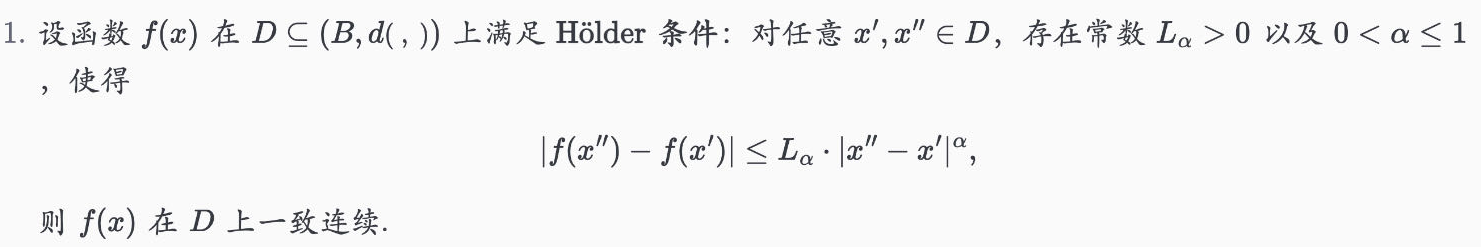
\includegraphics[width=\textwidth]{hw10-2025050821.png}
% \caption{}
\label{}
\end{figure}
\end{exercise}
For any $\epsilon>0$, put $\delta=\left( \frac{\epsilon}{L_{\alpha}} \right)^{1/\alpha}$, then
\[
\lvert f(x)-f(y) \rvert<\epsilon \qquad \forall \lvert x-y \rvert <\delta
\]
Thus $f$ is uniformly continuous on $D$.

\begin{exercise}
\begin{figure}[H]
\centering
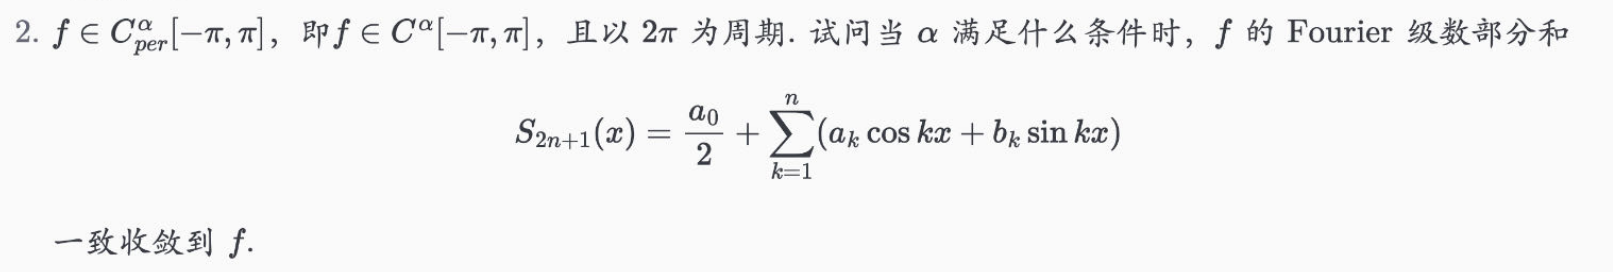
\includegraphics[width=\textwidth]{1-hw10-2025050821.png}
% \caption{}
\label{}
\end{figure}
\end{exercise}
\begin{note}
这个习题很有挑战性!
\end{note}
\begin{remark}
参见 Stein 习题 3.16 (d)
\begin{figure}[H]
\centering
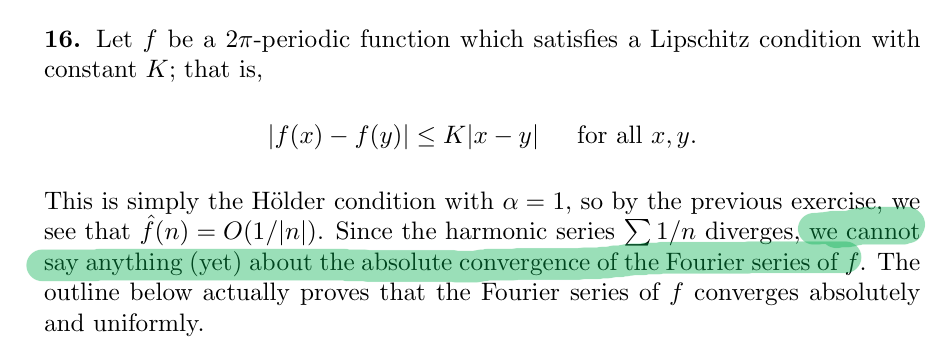
\includegraphics[width=\textwidth]{2-hw10-2025050822.png}
% \caption{}
\label{}
\end{figure}
\begin{figure}[H]
\centering
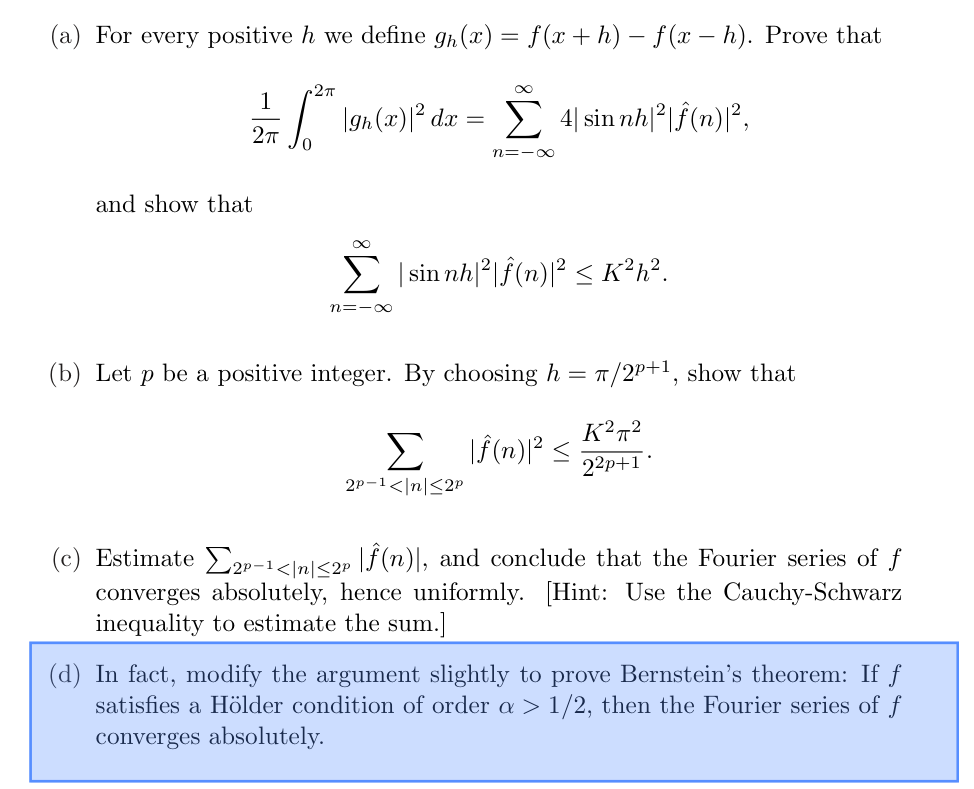
\includegraphics[width=\textwidth]{3-hw10-2025050822.png}
% \caption{}
\label{}
\end{figure}
\end{remark}
$\alpha>\frac{1}{2}$ 时一致收敛,$\alpha=\frac{1}{2}$ 时存在反例.

\begin{note}
反例参见《实分析中的反例》汪林
\begin{figure}[H]
\centering
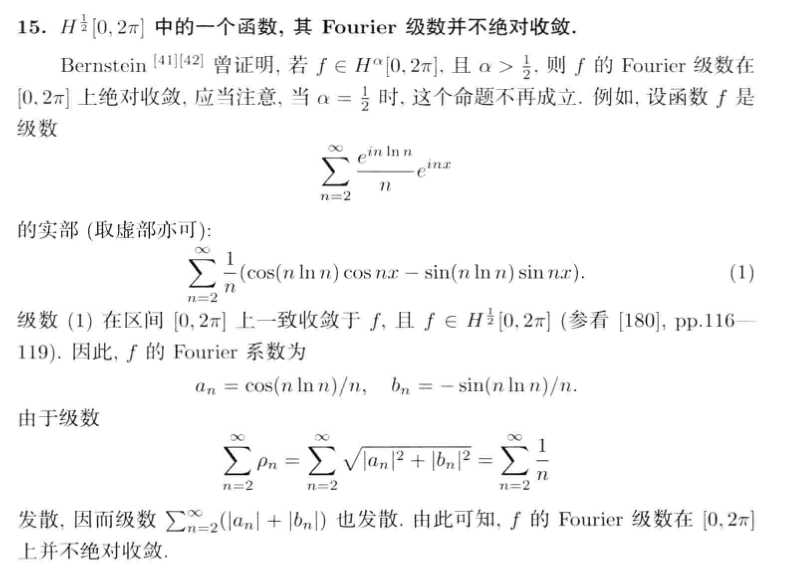
\includegraphics[width=\textwidth]{4-hw10-2025050822.png}
% \caption{}
\label{}
\end{figure}
\end{note}
证明太长了

\begin{figure}[H]
\centering
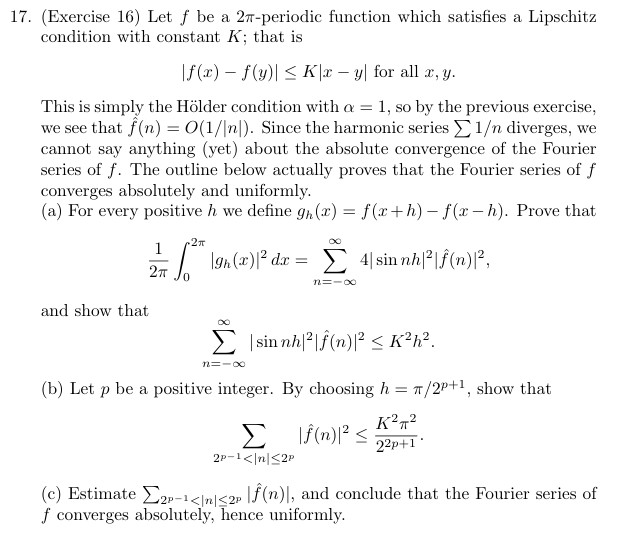
\includegraphics[width=\textwidth]{hw10-2025050823.png}
% \caption{}
\label{}
\end{figure}
\begin{figure}[H]
\centering
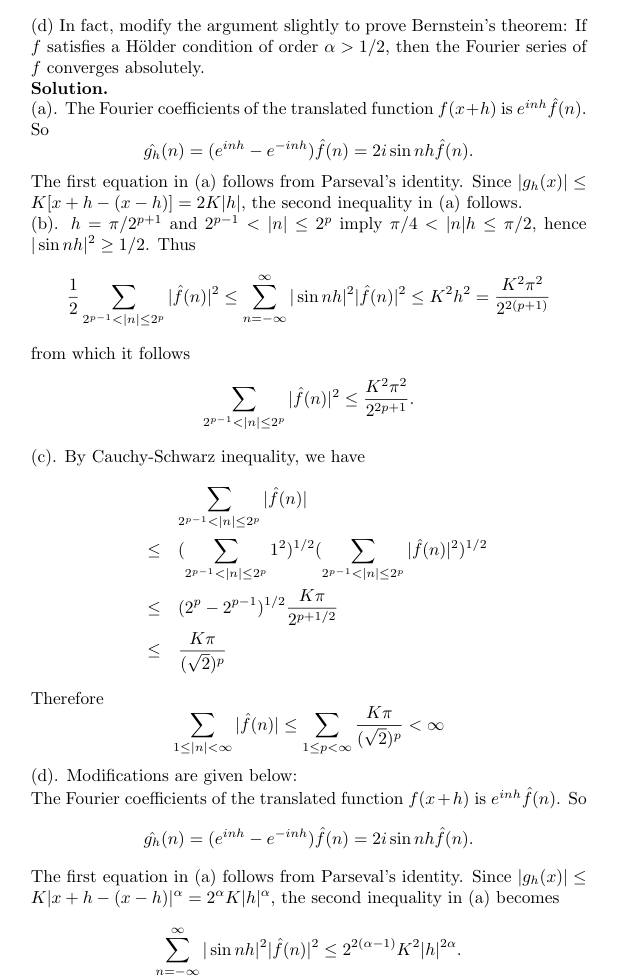
\includegraphics[width=\textwidth]{1-hw10-2025050823.png}
% \caption{}
\label{}
\end{figure}
\begin{figure}[H]
\centering
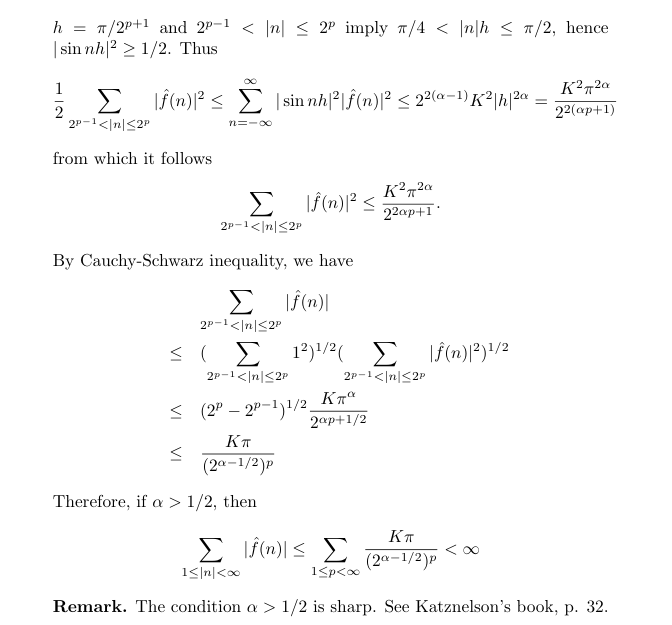
\includegraphics[width=\textwidth]{2-hw10-2025050823.png}
% \caption{}
\label{}
\end{figure}

A simpler version in Harmonic Analysis, Katznelson, p.33 :
\begin{figure}[H]
\centering
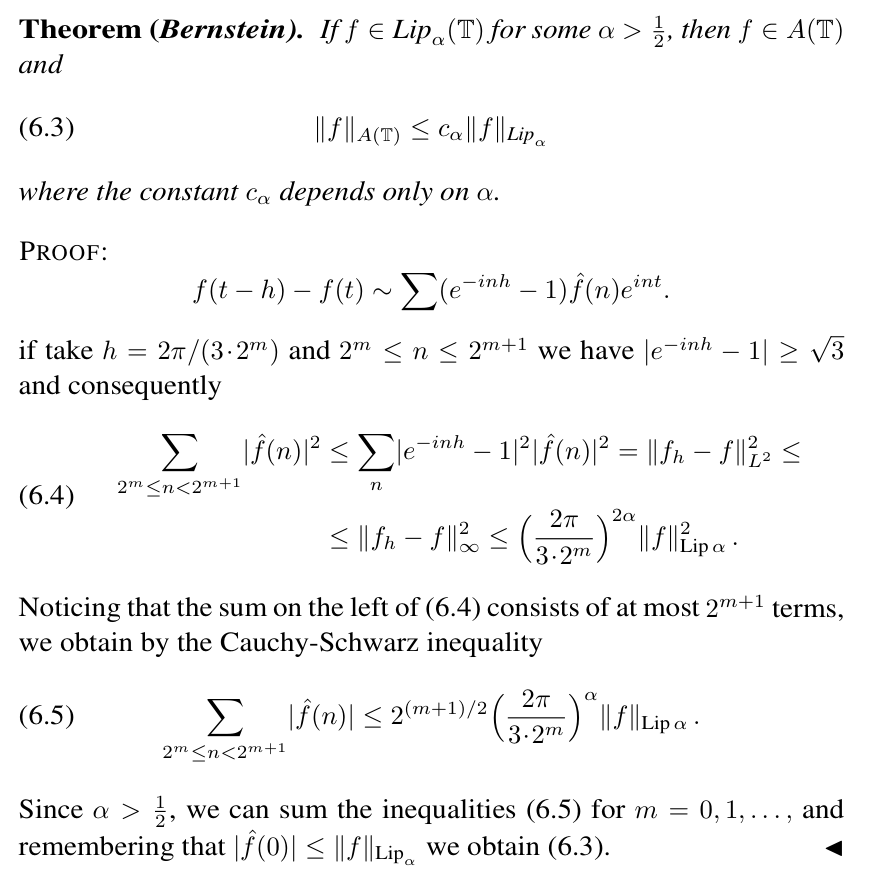
\includegraphics[width=\textwidth]{3-hw10-2025050823.png}
% \caption{}
\label{}
\end{figure}

\begin{exercise}
\begin{figure}[H]
\centering

\includegraphics[width=\textwidth]{2-hw10-2025050821.png}
% \caption{}
\label{}
\end{figure}
\end{exercise}
du Bois-Reymond showed an counterexample.

\begin{note}
参见于品《数学分析讲义 123》p.660
\begin{figure}[H]
\centering
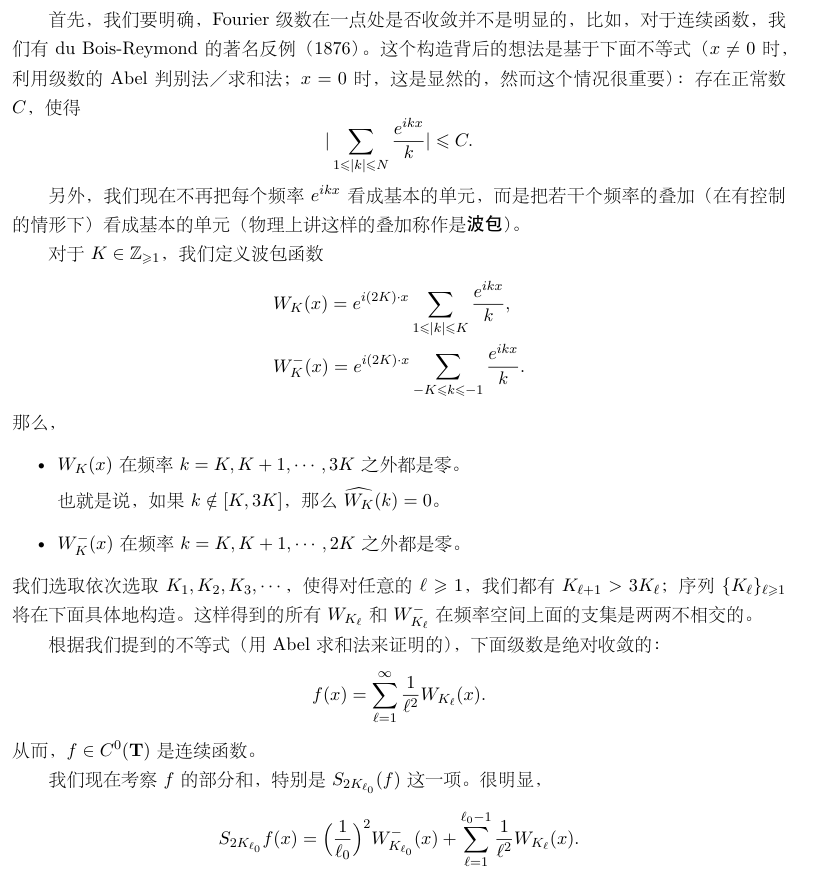
\includegraphics[width=\textwidth]{hw10-2025050822.png}
% \caption{}
\label{}
\end{figure}
\end{note}
\begin{figure}[H]
\centering
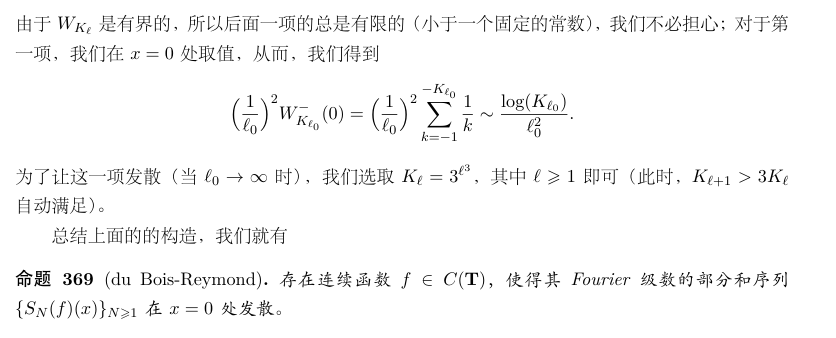
\includegraphics[width=\textwidth]{1-hw10-2025050822.png}
% \caption{}
\label{}
\end{figure}

\begin{exercise}
\begin{figure}[H]
\centering

\includegraphics[width=\textwidth]{3-hw10-2025050821.png}
% \caption{}
\label{}
\end{figure}
\end{exercise}
\begin{note}
题目可能出错了,$f(x)$ 在 $x\in[-1,0]$ 上无定义.
\end{note}
Since $x^{\frac{3}{2}}$ and $\sin\frac{1}{x}$ are continuous differentiable out of the neighborhood of 0, $f(x)$ is continuous differentiable.

For $x_0\in[-1,1]\setminus \{ 0 \}$,
\[
f'(x_0)=\frac{3}{2}x^{1/2 }\sin\frac{1}{x}-x^{-1/2 }\cos\frac{1}{x}
\]
For $x_0=0$,

\begin{exercise}
\begin{figure}[H]
\centering
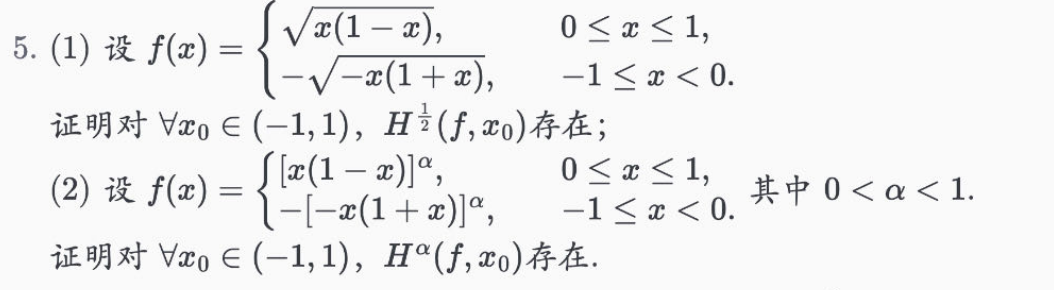
\includegraphics[width=\textwidth]{4-hw10-2025050821.png}
% \caption{}
\label{}
\end{figure}
\end{exercise}
$f(x)$ 在 $x_0$ 的 $\alpha$ 阶-Holder 常数定义为
\[
H^{\alpha}(f,x_0)\coloneqq \lim_{ \delta \to 0^{+} } \sup_{\lvert \Delta x \rvert <\delta}\frac{\lvert f(x_0+\Delta x)-f(x_0) \rvert }{\lvert \Delta x \rvert ^{\alpha}}
\]
这是 $\mathbb{R}^{1}$ 上导数定义的推广(推广到分数阶).

(1)
对于 $x_0\in(0,1)$,当 $\lvert \delta \rvert<\frac{x_0}{2}$ 时,
\[
\begin{aligned}
 \sup_{\lvert h \rvert <\delta}\frac{\lvert f(x_0+h)-f(x_0) \rvert }{\sqrt{ \lvert h \rvert  }} 
 & =   \sup_{\lvert h \rvert <\delta}\frac{\lvert \sqrt{ (x_0+h)(1-x_0-h) }-\sqrt{ x_0(1-x_0) } \rvert }{\sqrt{ \lvert h \rvert  }} \\
 & =   \sup_{\lvert h \rvert <\delta}\frac{\lvert h-2hx_0-h^2 \rvert }{\sqrt{ \lvert h \rvert  }(\sqrt{ (x_0+h)(1-x_0-h) }+\sqrt{ x_0(1-x_0) })} \\
 & \overset{\lvert \delta \rvert <\frac{x_0}{2}  }{ \leq  } \sup_{\lvert h \rvert <\delta}\frac{\sqrt{ \lvert h \rvert  }\lvert 1-2x_0-h \rvert }{\sqrt{ \frac{x_0}{2}\left( 1-\frac{x_0}{2} \right) }+\sqrt{ x_0(1-x_0) }} \\
 & \leq \sup_{\lvert h \rvert <\delta }\frac{3\sqrt{ \lvert h \rvert  } }{\sqrt{ \frac{x_0}{2}\left( 1-\frac{x_0}{2} \right) }+\sqrt{ x_0(1-x_0) }} \\
 & \leq  \frac{3\sqrt{ \lvert \delta \rvert  } }{\sqrt{ \frac{x_0}{2}\left( 1-\frac{x_0}{2} \right) }+\sqrt{ x_0(1-x_0) }}\to0 \qquad \text{as }\delta\to0 \\
\end{aligned}
\]
于是
\[
H^{\frac{1}{2}}(f,x_0)  =\lim_{ \delta \to 0^{+} } \sup_{\lvert h \rvert <\delta}\frac{\lvert f(x_0+h)-f(x_0) \rvert }{\sqrt{ \lvert h \rvert  }} =0
\]
类似的,对于 $x_0\in(-1,0)$,
\[
H^{\frac{1}{2}}(f,x_0)  =\lim_{ \delta \to 0^{+} } \sup_{\lvert h \rvert <\delta}\frac{\lvert f(x_0+h)-f(x_0) \rvert }{\sqrt{ \lvert h \rvert  }} =0
\]
当 $x_0=0$ 时,
\[
\sup_{\lvert h \rvert <\delta}\frac{\lvert f(h)-f(0) \rvert }{\sqrt{ \lvert h \rvert  }}=\sup_{\lvert h \rvert <\delta}\frac{\sqrt{ \lvert h \rvert (1-\lvert h \rvert ) }}{\sqrt{ \lvert h \rvert  }}=\sup_{\lvert h \rvert <\delta}\sqrt{ 1-\lvert h \rvert  }=\sqrt{ 1-\delta }
\]
于是
\[
H^{\frac{1}{2}}(f,0)=\lim_{ \delta \to 0^{+} } \sup_{\lvert h \rvert <\delta}\frac{\lvert f(h) -f(0)\rvert }{\sqrt{ \lvert h \rvert  }}=\lim_{ \delta \to 0^{+} } \sqrt{ 1-\delta }=1
\]
因此
\[
H^{\frac{1}{2}}(f,x_0)=\begin{cases}
1 & x_0=0 \\
0 & x_0\in[-1,0)\cup(0,1]
\end{cases}
\]
(2)
For $x_0\in(0,1)$, $\delta$ small enough
\[
\begin{aligned}
\sup_{\lvert h \rvert <\delta}\frac{\lvert f(x_0+h)-f(x_0) \rvert }{\lvert h \rvert ^{\alpha}} & =\sup_{\lvert h \rvert <\delta}\left\lvert  \frac{[(x_0+h)(1-x_0-h)]^{\alpha}-[x_0(1-x_0)]^{\alpha}}{\lvert h \rvert ^{\alpha}}   \right\rvert \\
 & =\sup_{\lvert h \rvert <\delta}\frac{[x_0(1-x_0)]^{\alpha}}{\lvert h \rvert ^{\alpha}}\left[ \left( 1-h\cdot\frac{h+2x_0-1}{x_0(1-x_0)} \right)^{\alpha}-1 \right] \\
 & =  \sup_{\lvert h \rvert <\delta}\frac{[x_0(1-x_0)]^{\alpha}}{\lvert h \rvert ^{\alpha}}\left( -\alpha h\cdot\frac{h+2x_0-1}{x_0(1-x_0)} +o(\delta^{2})\right) \\
 & =o(\delta^{1-\alpha})
\end{aligned}
\]
Thus
\[
H^{\alpha}(f,x_0)=\lim_{ \delta \to 0^{+} } o(\delta^{1-\alpha})=0
\]
Similarly, for $x_0\in[-1,0)$,
\[
H^{\alpha}(f,x_0)=0
\]
When $x_0=0$,
\[
\sup_{\lvert h \rvert <\delta}\frac{\lvert f(h)-f(0) \rvert }{\lvert h \rvert ^{\alpha}}=\sup_{\lvert h \rvert <\delta}\frac{[\lvert h \rvert (1-\lvert h \rvert )]^{\alpha}}{\lvert h \rvert ^{\alpha}}=\sup_{\lvert h \rvert <\delta}(1-\lvert h \rvert )^{\alpha}=(1-\delta)^{\alpha}
\]
Then
\[
H^{\alpha}(f,0)=\lim_{ \delta \to 0 } \sup_{\lvert h \rvert <\delta}\frac{\lvert f(h)-f(0) \rvert }{\lvert h \rvert ^{\alpha}}=\lim_{ \delta \to 0^{+} }(1-\delta)^{\alpha}=1
\]
Hence
\[
H^{\alpha}(f,x_0)=\begin{cases}
1 & x_0=0  \\
0 & x_0\in[-1,0)\cup(0,1]
\end{cases}
\]
\begin{exercise}
\begin{figure}[H]
\centering
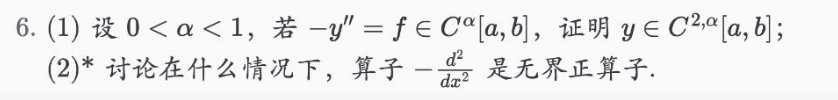
\includegraphics[width=\textwidth]{5-hw10-2025050822.png}
% \caption{}
\label{}
\end{figure}
\end{exercise}
若 $f' (x)\in C^{1}(D)$ 则称 $f (x)\in C^2(D)$;若还有 $f'' (x)\in C^{\alpha}(D)$,$0<\alpha\leq1$,则称 $f (x)\in C^{2,\alpha}(D)$.

由此,(1) 是显然的.

(2)

\begin{note}
Too hard.
\end{note}
选择合适的希尔伯特空间和带有合适边界条件的定义域(例如,Dirichlet条件下的$H_0^1(I) \cap H^2(I)$,或$L^2(\mathbb{R})$上的$H^2(\mathbb{R})$),算子$-\frac{d^2}{dx^2}$就是一个无界正算子。
